%%%%%%%%%%%%%%%%%%%%%%%%%%%%%%%%%%%%%%%%%
% Masters/Doctoral Thesis 
% LaTeX Template
% Version 1.43 (17/5/14)
%
% This template has been downloaded from:
% http://www.LaTeXTemplates.com
%
% Original authors:
% Steven Gunn 
% http://users.ecs.soton.ac.uk/srg/softwaretools/document/templates/
% and
% Sunil Patel
% http://www.sunilpatel.co.uk/thesis-template/
%
% License:
% CC BY-NC-SA 3.0 (http://creativecommons.org/licenses/by-nc-sa/3.0/)
%
% Note:
% Make sure to edit document variables in the Thesis.cls file
%
%%%%%%%%%%%%%%%%%%%%%%%%%%%%%%%%%%%%%%%%%

%----------------------------------------------------------------------------------------
%	PACKAGES AND OTHER DOCUMENT CONFIGURATIONS
%----------------------------------------------------------------------------------------

\documentclass[11pt, oneside]{Thesis} % The default font size and one-sided printing (no margin offsets)

\graphicspath{{Pictures/}} % Specifies the directory where pictures are stored

\usepackage[square, numbers, comma, sort&compress]{natbib} % Use the natbib reference package - read up on this to edit the reference style; if you want text (e.g. Smith et al., 2012) for the in-text references (instead of numbers), remove 'numbers' 

\usepackage{amsmath}
%\usepackage{amssymb}
\usepackage{graphicx}
%\usepackage{indentfirst}
%\usepackage{setspace}
%\doublespacing
%\usepackage{cite}
%\usepackage{hyperref}
%\usepackage{float}
\usepackage{notoccite}
%\usepackage{epstopdf}
%\usepackage{graphicx}
\usepackage{caption}
\usepackage{subcaption}
\usepackage{tabu}
\usepackage{multirow}
\usepackage{longtable}
\usepackage{array}
\usepackage{pifont}
\usepackage{hhline}
\usepackage{textcomp}
%\usepackage{gensymb}
\usepackage{breqn}
\usepackage{rotating}
\usepackage{float}

\hypersetup{urlcolor=blue, colorlinks=true} % Colors hyperlinks in blue - change to black if annoying
\title{\ttitle} % Defines the thesis title - don't touch this

\begin{document}

\frontmatter % Use roman page numbering style (i, ii, iii, iv...) for the pre-content pages

\setstretch{1.3} % Line spacing of 1.3

% Define the page headers using the FancyHdr package and set up for one-sided printing
\fancyhead{} % Clears all page headers and footers
\rhead{\thepage} % Sets the right side header to show the page number
\lhead{} % Clears the left side page header

\pagestyle{fancy} % Finally, use the "fancy" page style to implement the FancyHdr headers

\newcommand{\HRule}{\rule{\linewidth}{0.5mm}} % New command to make the lines in the title page

% PDF meta-data
\hypersetup{pdftitle={\ttitle}}
\hypersetup{pdfsubject=\subjectname}
\hypersetup{pdfauthor=\authornames}
\hypersetup{pdfkeywords=\keywordnames}

%----------------------------------------------------------------------------------------
%	TITLE PAGE
%----------------------------------------------------------------------------------------

%\begin{titlepage}
%\begin{center}
%
%\textsc{\LARGE \univname}\\[1.5cm] % University name
%\textsc{\Large Doctoral Thesis}\\[0.5cm] % Thesis type
%
%\HRule \\[0.4cm] % Horizontal line
%{\huge \bfseries \ttitle}\\[0.4cm] % Thesis title
%\HRule \\[1.5cm] % Horizontal line
% 
%\begin{minipage}{0.4\textwidth}
%\begin{flushleft} \large
%\emph{Author:}\\
%\href{http://www.johnsmith.com}{\authornames} % Author name - remove the \href bracket to remove the link
%\end{flushleft}
%\end{minipage}
%\begin{minipage}{0.4\textwidth}
%\begin{flushright} \large
%\emph{Supervisor:} \\
%\href{http://www.jamessmith.com}{\supname} % Supervisor name - remove the \href bracket to remove the link  
%\end{flushright}
%\end{minipage}\\[3cm]
% 
%\large \textit{A thesis submitted in fulfilment of the requirements\\ for the degree of \degreename}\\[0.3cm] % University requirement text
%\textit{in the}\\[0.4cm]
%\groupname\\\deptname\\[2cm] % Research group name and department name
% 
%{\large \today}\\[4cm] % Date
%%\includegraphics{Logo} % University/department logo - uncomment to place it
% 
%\vfill
%\end{center}
%
%\end{titlepage}

%----------------------------------------------------------------------------------------
%	DECLARATION PAGE
%	Your institution may give you a different text to place here
%----------------------------------------------------------------------------------------

%\Declaration{
%
%\addtocontents{toc}{\vspace{1em}} % Add a gap in the Contents, for aesthetics
%
%I, \authornames, declare that this thesis titled, '\ttitle' and the work presented in it are my own. I confirm that:
%
%\begin{itemize} 
%\item[\tiny{$\blacksquare$}] This work was done wholly or mainly while in candidature for a research degree at this University.
%\item[\tiny{$\blacksquare$}] Where any part of this thesis has previously been submitted for a degree or any other qualification at this University or any other institution, this has been clearly stated.
%\item[\tiny{$\blacksquare$}] Where I have consulted the published work of others, this is always clearly attributed.
%\item[\tiny{$\blacksquare$}] Where I have quoted from the work of others, the source is always given. With the exception of such quotations, this thesis is entirely my own work.
%\item[\tiny{$\blacksquare$}] I have acknowledged all main sources of help.
%\item[\tiny{$\blacksquare$}] Where the thesis is based on work done by myself jointly with others, I have made clear exactly what was done by others and what I have contributed myself.\\
%\end{itemize}
% 
%Signed:\\
%\rule[1em]{25em}{0.5pt} % This prints a line for the signature
% 
%Date:\\
%\rule[1em]{25em}{0.5pt} % This prints a line to write the date
%}
%
%\clearpage % Start a new page

%%----------------------------------------------------------------------------------------
%%	QUOTATION PAGE
%%----------------------------------------------------------------------------------------
%
%\pagestyle{empty} % No headers or footers for the following pages
%
%\null\vfill % Add some space to move the quote down the page a bit
%
%\textit{``Thanks to my solid academic training, today I can write hundreds of words on virtually any topic without possessing a shred of information, which is how I got a good job in journalism."}
%
%\begin{flushright}
%Dave Barry
%\end{flushright}
%
%\vfill\vfill\vfill\vfill\vfill\vfill\null % Add some space at the bottom to position the quote just right
%
%\clearpage % Start a new page
%
%%----------------------------------------------------------------------------------------
%%	ABSTRACT PAGE
%%----------------------------------------------------------------------------------------
%
%\addtotoc{Abstract} % Add the "Abstract" page entry to the Contents
%
%\abstract{\addtocontents{toc}{\vspace{1em}} % Add a gap in the Contents, for aesthetics
%
%The Thesis Abstract is written here (and usually kept to just this page). The page is kept centered vertically so can expand into the blank space above the title too\ldots
%}
%
%\clearpage % Start a new page

%%----------------------------------------------------------------------------------------
%%	ACKNOWLEDGEMENTS
%%----------------------------------------------------------------------------------------
%
%\setstretch{1.3} % Reset the line-spacing to 1.3 for body text (if it has changed)
%
%\acknowledgements{\addtocontents{toc}{\vspace{1em}} % Add a gap in the Contents, for aesthetics
%
%The acknowledgements and the people to thank go here, don't forget to include your project advisor\ldots
%}
%\clearpage % Start a new page



%% Title page: Manually formatted according to the university requirements.
\thispagestyle{empty} % No headers or page numbers

\begin{center}
\begin{figure}
  \begin{center}
    
\includegraphics[height=4cm]{asu_logo}
  \end{center}
\end{figure}
\small
\textbf{AIN SHAMS UNIVERSITY\\
	FACULTY OF ENGINEERING\\
	Computer Engineering and Systems}

%%Department%%

% Engineering Physics and Mathmatics
% Structural Engineering
% Irrigation and Hydraulics 
% Public Works 
% Architecture Engineering
% Urban Planning
% Electrical Power and Machines Engineering
% Electronics Engineering and Electrical Communications 
% Computer Engineering and Systems 
% Design and Production Engineering
% Mechanical Power Engineering
% Automotive Engineering
% Mechatronics Engineering

\vfill
\Large
\textbf{Metagenomic data analysis using deep learning} \\ 

\vfill
\small
A Thesis submitted in partial fulfillment of the requirements of \\ 
 Master of Science in Electrical Engineering  \\
(Computer Engineering and Systems)\\
%\vspace*{0.5cm}

%%Degree%%

% Master of Science
% Doctor of Philosophy

%%Branch%%

% Electrical Engineering
% Civil Engineering
% Mechanical Engineering 
% Architectural Engineering 
% Physics, Engineering Mathematics and Engineering Mechanics

%%Department%%

% Engineering Physics and Mathmatics
% Structural Engineering
% Irrigation and Hydraulics 
% Public Works 
% Architecture Engineering
% Urban Planning
% Electrical Power and Machines Engineering
% Electronics Engineering and Electrical Communications 
% Computer Engineering and Systems 
% Design and Production Engineering
% Mechanical Power Engineering
% Automotive Engineering
% Mechatronics Engineering


\vfill
\small
by\\
\large
\textbf{Aly O. Abdelkareem}\\
\small
Bachelor of Science in Electrical Engineering  \\
(Computer Engineering and Systems)\\
Faculty of Engineering, Ain Shams University, 2016\\

%%Last Degree%%

% Bachelor of Science
% Postrgaduate Diploma
% Master of Science

%%Branch%%

% Electrical Engineering
% Civil Engineering
% Mechanical Engineering 
% Architectural Engineering 
% Physics, Engineering Mathematics and Engineering Mechanics

%%Department%%

% Engineering Physics and Mathmatics
% Structural Engineering
% Irrigation and Hydraulics 
% Public Works 
% Architecture Engineering
% Urban Planning
% Electrical Power and Machines Engineering
% Electronics Engineering and Electrical Communications 
% Computer Engineering and Systems 
% Design and Production Engineering
% Mechanical Power Engineering
% Automotive Engineering
% Mechatronics Engineering

\vfill
\small
Supervised By\\
\normalsize
\textbf{Prof.~Hazem M. Abbas\\
	  Dr.~Mahmoud I. Khalil}

\vfill
\small
Cairo, 2018\\

\end{center}

\newpage
\thispagestyle{empty}
\mbox{}
\newpage
\thispagestyle{empty}
\newlength{\thenamewidth}
\newlength{\thesignaturewidth}
\newlength{\nameskip}

\setlength{\thenamewidth}{8cm}
\setlength{\thesignaturewidth}{4cm}
\setlength{\nameskip}{0.8cm}
%\vspace*{\fmtitlevoffset}


 \begin{center}
\begin{figure}
  \begin{center}
    
\includegraphics[height=4cm]{asu_logo}
  \end{center}
\end{figure}
\small


\textbf{AIN SHAMS UNIVERSITY\\
	FACULTY OF ENGINEERING\\
	Computer Engineering and Systems}

%%Department%%

% Engineering Physics and Mathmatics
% Structural Engineering
% Irrigation and Hydraulics 
% Public Works 
% Architecture Engineering
% Urban Planning
% Electrical Power and Machines Engineering
% Electronics Engineering and Electrical Communications 
% Computer Engineering and Systems 
% Design and Production Engineering
% Mechanical Power Engineering
% Automotive Engineering
% Mechatronics Engineering

\vfill
\Large
\textbf{Metagenomic data analysis using deep learning} \\ 

\vfill
\small

by\\
\large
\textbf{Aly O. Abdelkareem}\\
\small
Bachelor of Science in Electrical Engineering  \\
(Computer Engineering and Systems)\\
Faculty of Engineering, Ain Shams University, 2016\\

%%Last Degree%%

% Bachelor of Science
% Postrgaduate Diploma
% Master of Science

%%Branch%%

% Electrical Engineering
% Civil Engineering
% Mechanical Engineering 
% Architectural Engineering 
% Physics, Engineering Mathematics and Engineering Mechanics

%%Department%%

% Engineering Physics and Mathmatics
% Structural Engineering
% Irrigation and Hydraulics 
% Public Works 
% Architecture Engineering
% Urban Planning
% Electrical Power and Machines Engineering
% Electronics Engineering and Electrical Communications 
% Computer Engineering and Systems 
% Design and Production Engineering
% Mechanical Power Engineering
% Automotive Engineering
% Mechatronics Engineering


%\vspace*{\fmtitlevskip}


\vspace{3em}
\textbf{Examiners' Committee}

\end{center} 

\begin{tabular}{lr}
	\textbf{Name and affiliation}	& \textbf{Signature}\\

%\begin{minipage}{\thenamewidth}
%\vspace{\nameskip}
%\small\textbf{Prof. Dr. }\\
%\small , \\
%\small Faculty of Engineering,\\
%\small Electronics \& Communications Dept.
%\end{minipage}
%&
%\begin{minipage}{\thesignaturewidth}
%	\dotfill \hspace{0.1\thesignaturewidth}
%\end{minipage} \\
%\hline
\begin{minipage}{\thenamewidth}
\vspace{\nameskip}
\small\textbf{Prof.~}\\
\small Computer Engineering and Systems\\
\small Faculty of Engineering, Ain Shams University. \\
\end{minipage}
&
\begin{minipage}{\thesignaturewidth}
	\dotfill \hspace{0.1\thesignaturewidth}
\end{minipage} \\
%\hline

\begin{minipage}{\thenamewidth}
\vspace{\nameskip}
\small\textbf{Prof.~}\\
\small Computer Engineering and Systems\\
\small Faculty of Engineering, Ain Shams University. \\
\end{minipage}
&
\begin{minipage}{\thesignaturewidth}
	\dotfill \hspace{0.1\thesignaturewidth}
\end{minipage} \\
%\hline

\begin{minipage}{\thenamewidth}
\vspace{\nameskip}
\small\textbf{Dr.~}\\
\small Choose Department\\
\small Faculty of Engineering, University. \\
\end{minipage}
&
\begin{minipage}{\thesignaturewidth}
	\dotfill \hspace{0.1\thesignaturewidth}
\end{minipage} \\
%\hline

%%Department%%

% Engineering Physics and Mathmatics
% Structural Engineering
% Irrigation and Hydraulics 
% Public Works 
% Architecture Engineering
% Urban Planning
% Electrical Power and Machines Engineering
% Electronics Engineering and Electrical Communications 
% Computer Engineering and Systems 
% Design and Production Engineering
% Mechanical Power Engineering
% Automotive Engineering
% Mechatronics Engineering

\end{tabular}

\begin{flushright}
\large
Date:25  Feb 2019
\end{flushright}
\newpage
\thispagestyle{empty}
\mbox{}
%-----------------------------------------
% Statement(manually formatted)
%-----------------------------------------
\setlength{\thesignaturewidth}{2cm}
\newpage
\thispagestyle{empty}
%\vspace*{\fmtitlevoffset}
\begin{center}\huge\textbf{Statement}\end{center}
%\vspace*{\fmtitlevskip}
\Large
\vfill
This thesis is submitted as a partial fulfillment of Master of Science in Electrical Engineering, Faculty of Engineering, Ain Shams University.
The author carried out the work included in this thesis, and no part of it has been submitted for a degree or a qualification at any other scientific entity. 

%%Degree%%

% Master of Science
% Doctor of Philosophy

%%Branch%%

% Electrical Engineering
% Civil Engineering
% Mechanical Engineering 
% Architectural Engineering 
% Physics, Engineering Mathematics and Engineering Mechanics


\vfill
%\vspace{\fmtitlevskip}
\begin{flushright}
\large
\textbf{Aly O. Abdelkareem} \\

\small
Signature \\
\dotfill \hspace{0.1\thesignaturewidth}

\textbf{Date:} 25 Dec 2018 \\
\end{flushright}
\vfill

\normalsize

\newpage
\thispagestyle{empty}
\mbox{}
% Settings for Preliminary Pages
\newpage
\thispagestyle{empty}
%\pagestyle{plain} % No headers, just page numbers
%\setcounter{page}{2}

%-----------------------------------------
% Curriculum Vitae(manually formatted)
%-----------------------------------------
\begin{center}\huge \textbf{Researcher Data}\end{center}
%\large
\vspace{3em}
\begin{flushleft}
\textbf{Name:} Aly Osama Aly Ibrahim Abdelkareem (Aly O. Abdelkareem)\\

\textbf{Date of Birth:} 29/08/1992 \\

\textbf{Place of Birth:} Cairo, Egypt \\

\textbf{Last academic degree:} Bachelor of Science in Electrical Engineering \\

\textbf{Field of specialization:} Computer Engineering and Software Systems (Credit Hours) \\

\textbf{University issued the degree	:}  Ain Shams University\\

\textbf{Date of issued degree	:} 15/6/2016 \\


\textbf{Current job		:} Teaching and Research Assistant at Faculty of Engineering\\

\end{flushleft}
\vfill


%%Last Degree%%

% Bachelor of Science
% Postrgaduate Diploma
% Master of Science
\newpage
\thispagestyle{empty}
\mbox{}
% Settings for Preliminary Pages
\newpage
\thispagestyle{empty}
%\pagestyle{plain} % No headers, just page numbers
%\setcounter{page}{2}

%-----------------------------------------

%-----------------------------------------
\begin{center}\huge \textbf{Thesis Summary}\end{center}


\begin{center}
\underline{\textbf{Summary}}
\end{center}
%
The thesis is divided into seven chapters as listed below:
%
\begin{flushleft}
\underline{Chapter 1}
\end{flushleft}
%
%
%
%
\begin{flushleft}
\underline{Chapter 2}
\end{flushleft}
%
%
%
\begin{flushleft}
\underline{Chapter 3}
\end{flushleft}
%
%
%
\begin{flushleft}
\underline{Chapter 4}
\end{flushleft}
%
%
%
%
\begin{flushleft}
\underline{Chapter 5}
\end{flushleft}
%
%
%
\begin{flushleft}
\underline{Chapter 6}
\end{flushleft}
%
%
%
\begin{flushleft}
\underline{Chapter 7}
\end{flushleft}



\begin{flushleft}
\large

Key words: bioinformatics, classification, deep learning, metagenomics
\end{flushleft}




\newpage
\thispagestyle{empty}
\mbox{}
%% $Log: abstract.tex,v $
% Revision 1.1  93/05/14  14:56:25  starflt
% Initial revision
% 
% Revision 1.1  90/05/04  10:41:01  lwvanels
% Initial revision
% 
%
%% The text of your abstract and nothing else (other than comments) goes here.
%% It will be single-spaced and the rest of the text that is supposed to go on
%% the abstract page will be generated by the abstractpage environment.  This
%% file should be \input (not \include 'd) from cover.tex.
%\pagenumbering{gobble}
\clearpage
\thispagestyle{empty}
\chapter*{Abstract}
\addcontentsline{toc}{chapter}{Abstract}

\begin{center}
\textbf{Faculty of Engineering – Ain Shams University\\
Electronics and Communication Engineering Department }
\end{center}

\begin{flushleft}
Thesis title: \textbf{""} \\

Submitted by: \textbf{} \\

Degree: \textbf{} \\
\end{flushleft}

\begin{center}
\underline{\textbf{Abstract}}
\end{center}



% Settings for Preliminary Pages
\newpage
\thispagestyle{empty}
%\pagestyle{plain} % No headers, just page numbers
%\setcounter{page}{2}

%-----------------------------------------
% Curriculum Vitae(manually formatted)
%-----------------------------------------
\begin{center}\huge \textbf{Acknowledgment}\end{center}
%\large

\begin{flushright}
\large
Aly O. Abdelkareem\\
Computer Engineering and Systems\\
Faculty of Engineering\\
Ain Shams University\\
Cairo, Egypt\\
Dec 2018
\end{flushright}



I would like to express my sincere gratitude to my mother and my father for the continuous support of my study, my wife Mayada for her patience and motivation, and my daughter Aisha as she brought happiness to my life.



%%Department%%

% Engineering Physics and Mathmatics
% Structural Engineering
% Irrigation and Hydraulics 
% Public Works 
% Architecture Engineering
% Urban Planning
% Electrical Power and Machines Engineering
% Electronics Engineering and Electrical Communications 
% Computer Engineering and Systems 
% Design and Production Engineering
% Mechanical Power Engineering
% Automotive Engineering
% Mechatronics Engineering



%----------------------------------------------------------------------------------------
%	LIST OF CONTENTS/FIGURES/TABLES PAGES
%----------------------------------------------------------------------------------------

\pagestyle{fancy} % The page style headers have been "empty" all this time, now use the "fancy" headers as defined before to bring them back

\lhead{\emph{Table of Contents}} % Set the left side page header to "Table of Contents"
\tableofcontents % Write out the Table of Contents

\lhead{\emph{List of Figures}} % Set the left side page header to "List of Figures"
\listoffigures % Write out the List of Figures

\lhead{\emph{List of Tables}} % Set the left side page header to "List of Tables"
\listoftables % Write out the List of Tables

%----------------------------------------------------------------------------------------
%	ABBREVIATIONS
%----------------------------------------------------------------------------------------

\clearpage % Start a new page

\setstretch{1.5} % Set the line spacing to 1.5, this makes the following tables easier to read

\lhead{\emph{List of Abbreviations}} % Set the left side page header to "List of Abbreviations"
\listofsymbols{ll} % Include a list of Abbreviations (a table of two columns)
{
\textbf{LAH} & \textbf{L}ist \textbf{A}bbreviations \textbf{H}ere \\
%\textbf{Acronym} & \textbf{W}hat (it) \textbf{S}tands \textbf{F}or \\
}

%----------------------------------------------------------------------------------------
%	PHYSICAL CONSTANTS/OTHER DEFINITIONS
%----------------------------------------------------------------------------------------

%\clearpage % Start a new page
%
%\lhead{\emph{Physical Constants}} % Set the left side page header to "Physical Constants"
%
%\listofconstants{lrcl} % Include a list of Physical Constants (a four column table)
%{
%Speed of Light & $c$ & $=$ & $2.997\ 924\ 58\times10^{8}\ \mbox{ms}^{-\mbox{s}}$ (exact)\\
%% Constant Name & Symbol & = & Constant Value (with units) \\
%}

%----------------------------------------------------------------------------------------
%	SYMBOLS
%----------------------------------------------------------------------------------------

\clearpage % Start a new page

\lhead{\emph{List of Symbols}} % Set the left side page header to "List of Symbols"

\listofnomenclature{lll} % Include a list of Symbols (a three column table)
{
$a$ & distance & m \\
$P$ & power & W (Js$^{-1}$) \\
% Symbol & Name & Unit \\

& & \\ % Gap to separate the Roman symbols from the Greek

$\omega$ & angular frequency & rads$^{-1}$ \\
% Symbol & Name & Unit \\
}

%----------------------------------------------------------------------------------------
%	DEDICATION
%----------------------------------------------------------------------------------------
%
%\setstretch{1.3} % Return the line spacing back to 1.3
%
%\pagestyle{empty} % Page style needs to be empty for this page
%
%\dedicatory{For/Dedicated to/To my\ldots} % Dedication text
%
%\addtocontents{toc}{\vspace{2em}} % Add a gap in the Contents, for aesthetics

%----------------------------------------------------------------------------------------
%	THESIS CONTENT - CHAPTERS
%----------------------------------------------------------------------------------------

\mainmatter % Begin numeric (1,2,3...) page numbering

\pagestyle{fancy} % Return the page headers back to the "fancy" style

% Include the chapters of the thesis as separate files from the Chapters folder
% Uncomment the lines as you write the chapters

% Chapter 1

\chapter{Introduction} % Main chapter title

\label{Chapter1} % For referencing the chapter elsewhere, use \ref{Chapter1} 

\lhead{Chapter 1. \emph{Introduction}} % This is for the header on each page - perhaps a shortened title

%----------------------------------------------------------------------------------------

\section{Metagenomic analysis}

\subsection{Definition}

{M}{etagenomics} is an analysis of the genetic information of the collective genomes of the microbes within a given environment based on its sampling regardless of cultivability of the cells. \cite{izard2014metagenomics}. There is a minor population of microbial organisms identified due to the difficulty in studying them using pure culture isolation. This methodology has been constrained to less than 1\% of host cells and is biased to certain species \cite{labonte2015single}.
% https://www.the-scientist.com/daily-news/most-gut-microbes-can-be-cultured-33581
Metagenomic analysis process demonstrates a promising understanding of different microorganisms. It answers some questions about the identity of microorganisms in the collection and their potential functional characterization.

\subsection{Microorganism}


Microorganisms are found everywhere on earth, and they are critical in our survival. This study, our interest is in prokaryotic microorganisms (e.g. bacteria and archaea) and viruses. Bacteria are unicellular and microscopic organisms that reproduce by binary fission. On the other hand, viruses are typically submicroscopic consists of genetic materials either DNA or RNA surrounded by a protective coat of proteins and can only replicate inside living host cells. They lack metabolic enzymes and translational machinery such as ribosomes for making proteins. There are 200 to a few thousand genes in the bacterial genomes, while the tiniest viral genomes have only three genes and the largest have up to 2000 genes.


\section{Viruses}


\subsection{Definition}

Viruses have an impact on different microbial communities, and virus-host interaction can change many ecosystems such as human health and aquatic life. Phages or bacteriophages are viruses that infect bacteria. Furthermore, phages are abundant in different microbiome communities. The viral infection starts when virus binds to a host cell and its genome integrates with the host cell genome. The integrated viral DNA is called a provirus. It is reasonable to think that isolated viruses are just package of genes moving from one host cell to another.

\subsection{Importance in clinical and environment}

very very important.

\subsection{Identification}

 Scientists are using isolation and culturing techniques to study viral diversity and viral-host interactions in microbial communities. Those techniques have many limitations because there is no universal marker gene for viruses. The sequenced viruses in NCBI RefSeq database constitute approximately 5\% of known species of prokaryotic organisms \cite{roux2015viral}.

\section{Next Generation Sequencing}

High throughput sequencing technology is used for metagenomic studies which can generate large number of read  sequences of microorganisms. The expected read length is up to 600 bp and the number of generated reads per run is up to 15 million approximately based on the sequencing platform and the library preparation methods \cite{allali2017comparison}. We can sequence mixture of prokaryotic cells and viruses in complex microbial communities in a cultivation-independent process. Sequencing of microbial samples shows contamination of viral sequences within prokaryotic population. A study found 4-17\% virus sequences in human gut prokaryotic metagenomes \cite{minot2011human}. Moreover, cellular contamination is quite frequent even with a careful purification of viral particles, and this is one of the main reasons why we need a tool that can differentiate between bacterial and viral sequences.

\subsection{Sequencer Tools}

different tools of HTS
\subsection{Data types}
different types of data

\subsection{Sequence identification in HTS}


The broadly adopted technique to know who is in metagenomic data is to assemble the high throughput reads to contigs then search against a known genomic database using sequence alignment method in order to infer the type of microorganisms and the existence of species in a metagenomic sample. This approach is minimal because it only detects viruses almost related to those we already know. It is reported that about 15\% of viruses in the human gut microbiome and 10\% in the ocean have similarity to the known viruses \cite{ren2017virfinder}. 

\section{Machine learning}

Machine learning approaches have been used to classify and cluster data based on extracted features. The deep neural network is one of machine learning methods that are considered as a state of the art category for general classification problems. Deep learning shows significant improvements in several artificial intelligence tasks for example image classification, speech recognition, and natural language processing. Moreover, It shows significant results with genomic data \cite{angermueller2016deep}. %\\

\section{Our Contribution}

In this paper, we introduce a deep sequence model, VirNet, to identify viral reads from a mixture of viral and bacterial sequences and purify viral metagenomic data from bacterial contamination as well. That will guide us to identify new viruses and potentially perform functional characterization. Additionally, it will answer many mysteries related to our understanding of their functionality and diversity in the ecosystem.


% Chapter 2

\chapter{Related Work} % Main chapter title

\label{Chapter2} % For referencing the chapter elsewhere, use \ref{Chapter1} 

\lhead{Chapter 2. \emph{Related Work}} % This is for the header on each page - perhaps a shortened title

%----------------------------------------------------------------------------------------

There has been extensive prior work on viral identification. Recent work has focused on identifying phages in bacterial genomes. Several methods have used similarity search by sequence alignment with the reference genomes in order to find viral contigs. Most of the recent tools fall under three categories based on the sample structure such as:
\begin{enumerate}
	\item phages from prokaryotic genomes
	\item viral sequences in mixed metagenomic datasets
	\item phages and viral sequences. 
\end{enumerate} 

\section{Similarity tools}

There are many software packages to find phages from prokaryotic genomes such as Phage\_Finder \cite{fouts2006phage_finder}, Prophinder \cite{lima2008prophinder}, PHAST\cite{zhou2011phast}, and PhiSpy \cite{akhter2012phispy}. These tools are using similarity search to known virus databases using features such as genes. Some of them such as PhiSpy integrates other features such as  unique virus k-mers, AT and GC skew, protein length and transcription strand direction. They have many limitations as they failed to detect viral sequences in metagenomic data as the databases are outdated, limited and don't represent viral diversity in the environment. Moreover, It is not optimized to process a large number of contigs \cite{roux2015virsorter} as they depend on alignment and homology processing limitations. 

The second category is able to detect viral sequences in mixed metagenomic datasets such as VIROME \cite{wommack2012virome} and MetaVir\cite{roux2011metavir}. They are using similarity search with the databases same as the first category. Additionally, they are searching against proteins. There are more packages such as DIAMOND \cite{buchfink2014Diamond} or Centrifuge \cite{kim2016centrifuge} which are much faster and efficient than the former tools for microbial classification. Again, The limitation of this approach is using limited known reference databases. 
%----------------------------------------------------------------------------------------

\section{Statistical tools}


The third category of software packages such as VirSorter \cite{roux2015virsorter} is able to detect phages and viral sequences. VirSorter is using similarity search to viral databases and integrates other features related to analysis of sequence genes such as enrichment of viral-like genes, enrichment of uncharacterized genes and viral hallmark gene. These features make the identification more accurate but it still suffer limitations. One of the limitations is the requirements of having at least 3 genes within the contig because the smallest virus genome contains 3 genes because the smallest virus discovered has 3 genes only so it has the same limitations as previous techniques because of using homology strategy. Moreover, it cannot work with short fragments or contigs and it is very slow in processing metagenomic datasets. 

Recently VirFinder \cite{ren2017virfinder} applied machine learning techniques. VirFinder is a statistical method based on the logistic regression model. It uses the K-mer feature which is considered as a discrimination feature for different sequence problems. It shows a great success with short sequences too and They found a great k-mer similarity score with viruses within other prokaryotic genomes. 

% need to write deep learning techniques in fragments classification

In this paper, we are using deep learning techniques which is much more suitable to sequence problems and also shows significant improvements to other current machine learning models. In deep neural networks, the model will extract the most appropriate features during training which lead to better identification accuracy and sensitivity. 

 
% Chapter 3

\chapter{Deep neural networks for identification} % Main chapter title

\label{Chapter3} % For referencing the chapter elsewhere, use \ref{Chapter1} 

\lhead{Chapter 3. \emph{Deep neural networks for identification}} % This is for the header on each page - perhaps a shortened title

%----------------------------------------------------------------------------------------



\section{Sequence neural networks}

Recurrent neural networks (RNN), long short-term memory (LSTM) \cite{hochreiter1997long} and gated recurrent neural networks (GRU) \cite{chung2014empirical} can model complex sequences and have been used for sequence modeling problems.

Our deep learning model is implemented as an attentional encoder network (Figure \ref{fig:encoder}). An input sequence  $\mathbf{x = (x_{1} , \ldots{} , x_{m} )}$  and calculates a forward sequence of hidden states  ($\mathbf{\overrightarrow{h_{1}}}$,\ldots{},$\mathbf{ \overrightarrow{h_{m}}}$). The hidden states $\mathbf{\overrightarrow{h_{j}}}$  are averaged to obtain the attention vector $\mathbf{h_{j}}$ representing the context vector from the input sequence.

Embedding layer maps discrete input words to dense vectors for computational efficiency before feeding this sequence to LSTM/GRU Layers. The attentional network could learn how to extract suitable features from the raw data and can attend to previous DNA nucleotide within the same input sequence. 

LSTM encoder have 3 gates to protect and control the cell state, the input gate denoted $\mathbf{i}$ which defines how much of the newly computed state you want to let through, forget gate denoted $\mathbf{f}$ that decides what information is to be kept and what is to be thrown away,  the output of the update gate denoted $\mathbf{U}$ that's used to update the cell state and the output of the LSTM cell $\mathbf{o}$ .$\mathbf{W}$ is the recurrent connection at the previous hidden layer and current hidden layer and $\mathbf{C}$ is the internal memory of the unit  as shown in the following equations \newline
$\mathbf{i_{t}=\sigma(x_{t}U^i + h_{t-1}W^i)}$ \newline
$\mathbf{f_{t}=\sigma(x_{t}U^f + h_{t-1}W^f)}$ \newline
$\mathbf{o_{t}=\sigma(x_{t}U^o + h_{t-1}W^o)}$. 

GRU encoder is same as LSTM except it has only 2 gates, Reset gate denoted $\mathbf{r}$ that determines how to combine the new input with the previously saved input state and the update gate denoted $\mathbf{z}$ that defines the amount of information to keep around, as defined  in the following equations \newline
$\mathbf{z_{t}=\sigma(x_{t}U^z + h_{t-1}W^z)}$ \newline
$\mathbf{r_{t}=\sigma(x_{t}U^r + h_{t-1}W^r)}$ \newline
$\mathbf{\overline{h_{t}} = tanh(x_{t}U^h + (r_{t} * h_{t-1})W^h )}$ \newline
$\mathbf{ h_{t} = (1-z_{t})h_{t-1} +z_{t}\overline{h_{t}}}$.


The attentional neural model was trained with the DNA nucleotide bases with fragments with different lengths. The model will predict in a binary output format whether this fragment is viral or non-viral.

The top-performing model (Figure \ref{fig:model_diagram}) consists of an input embedding layer of size 128 mapping input DNA nucleotide tokens into an embedding space, that is fed to an LSTM layer. The forward sequence $\mathbf{\overrightarrow{h_{j}}}$ is then averaged together to create an attentional vector representing token context within the same fragment. A dropout layer was added after the attentional layer to avoid overfitting over the input data.

LSTM layer was performing better as in \ref{table:hyper_results} than the GRU cell. GRU encoder having less gates than LSTM model make it faster and easier to converge, but depedending on the size and the format of the input data. LSTM with more gates would be slower but will outperform GRU encoder type.

The input sequence is divided into 5 grams sized tokens these tokens are then treated as a single word (Figure \ref{fig:encoder}). This single token is mapped as a point in the embedding space created during training the neural model.

During training, all parameters are optimized jointly using Adam to maximize the conditional probability of tokens found together to predict if an input sequence is viral or not.

In this model, an early stopping mechanism was used as a form of regularization to avoid over-fitting over the data while making more epochs over the data. The early stopping mechanism was used with patience of 3 non -improving consecutive epochs; the neural model will stop training while saving the latest improving checkpoint over the validation set defined.

\subsection{Attention mechanism}


\LaTeX{} is not a WYSIWYG (What You See is What You Get) program, unlike word processors such as Microsoft Word or Apple's Pages. Instead, a document written for \LaTeX{} is actually a simple, plain text file that contains \emph{no formatting}. You tell \LaTeX{} how you want the formatting in the finished document by writing in simple commands amongst the text, for example, if I want to use \textit{italic text for emphasis}, I write the `$\backslash$\texttt{textit}\{\}' command and put the text I want in italics in between the curly braces. This means that \LaTeX{} is a ``mark-up'' language, very much like HTML.

\section{Convolution neural networks}

\LaTeX{} is not a WYSIWYG (What You See is What You Get) program, unlike word processors such as Microsoft Word or Apple's Pages. Instead, a document written for \LaTeX{} is actually a simple, plain text file that contains \emph{no formatting}. You tell \LaTeX{} how you want the formatting in the finished document by writing in simple commands amongst the text, for example, if I want to use \textit{italic text for emphasis}, I write the `$\backslash$\texttt{textit}\{\}' command and put the text I want in italics in between the curly braces. This means that \LaTeX{} is a ``mark-up'' language, very much like HTML.

\subsection{Triplet loss mechanism}


\LaTeX{} is not a WYSIWYG (What You See is What You Get) program, unlike word processors such as Microsoft Word or Apple's Pages. Instead, a document written for \LaTeX{} is actually a simple, plain text file that contains \emph{no formatting}. You tell \LaTeX{} how you want the formatting in the finished document by writing in simple commands amongst the text, for example, if I want to use \textit{italic text for emphasis}, I write the `$\backslash$\texttt{textit}\{\}' command and put the text I want in italics in between the curly braces. This means that \LaTeX{} is a ``mark-up'' language, very much like HTML.

%----------------------------------------------------------------------------------------



\subsection{Hyperparameters optimization}

Model parameters affect the performance of the deep learning model, and they control the behavior of the training algorithm as well. We selected the grid search technique in order to find the most suitable parameters. The grid search is considered a traditional technique for hyperparameters optimization and it brute force different combinations. We ran several experiments on 20\% of our training set for 500 bp. Then, we divided it into training, validation, and testing set with the following percentages 70\%, 10\%, and 20\%. These experiments were designed to find the best parameters for the number of recurrent layers, the embedding size for each layer and the input sub-words (ngram). Our reported results (Table \ref{table:hyper_results}) show that the best parameters setup is for 2 layers, 128 embedding size, and 5 ngram. 

We ran other experiments with the same parameters to check the ability of our model with other configuration, so we changed different parameters separately such as embedding size to 256 neurons, the number of layers to 3 and the recurrent cell type to GRU instead of LSTM. We found a slightly less accuracy and ROC-AUC scores but the training time was much more than the best parameters configuration as expected due to increasing number of neural network parameters.

\begin{table}[!htbp]
	\centering
	\begin{tabular}{||c c c c c||} 
		\#Layers & Embedding & Ngram & ROC-AUC & Accuracy \\ [0.5ex] 
		\hline\hline
		1      & 32                      & 3     & 0.8     & 73.66    \\
		1      & 32                      & 5     & 0.83    & 76.42    \\
		1      & 32                      & 7     & 0.79    & 72.11    \\
		1      & 64                      & 3     & 0.83    & 76.1     \\
		1      & 64                      & 5     & 0.83    & 75.98    \\
		1      & 64                      & 7     & 0.77    & 69.96    \\
		1      & 128                     & 3     & 0.83    & 75.76    \\
		1      & 128                     & 5     & 0.85    & 77.41    \\
		1      & 128                     & 7     & 0.78    & 70.93    \\
		2      & 32                      & 3     & 0.8     & 73.25    \\
		2      & 32                      & 5     & 0.83    & 76.49    \\
		2      & 32                      & 7     & 0.79    & 72.82    \\
		2      & 64                      & 3     & 0.81    & 73.96    \\
		2      & 64                      & 5     & 0.84    & 76.46    \\
		2      & 64                      & 7     & 0.78    & 72.53    \\
		2      & 128                     & 3     & 0.83    & 76.15    \\
		\textbf{2} & \textbf{128}            & \textbf{5} & \textbf{0.85} & \textbf{77.9} \\
		2      & 128                     & 7     & 0.78    & 70.63    \\[1ex]
	\end{tabular}
	\caption{Hyperparamters optimization results}
	\label{table:hyper_results}
\end{table}


\begin{figure}[!htbp]
	\centering
	\begin{subfigure}{0.5\textwidth}
		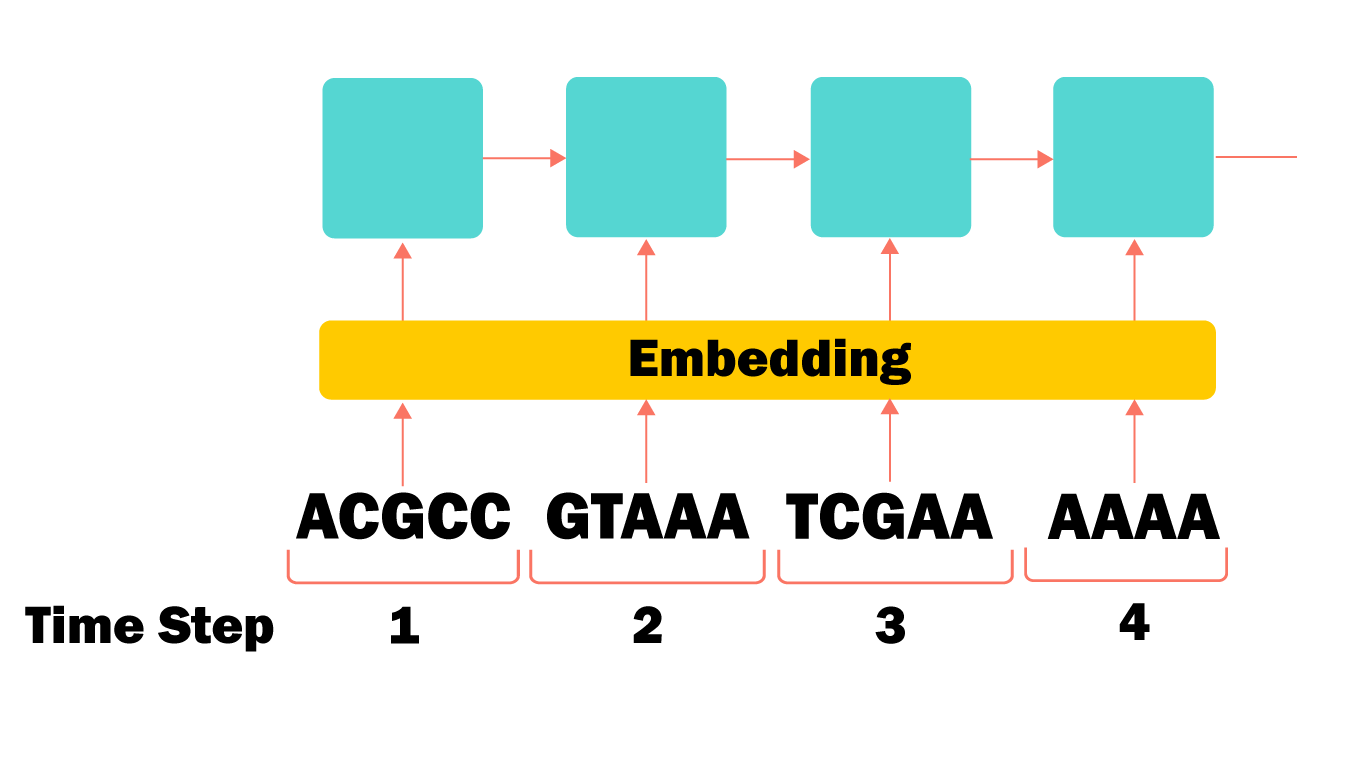
\includegraphics[width=\linewidth]{Pictures/encoder.PNG}
		\caption{Embedding Layer} 
		\label{fig:encoder}
	\end{subfigure}
	\hspace*{\fill} % separation between the subfigures
	\begin{subfigure}{0.5\textwidth}
		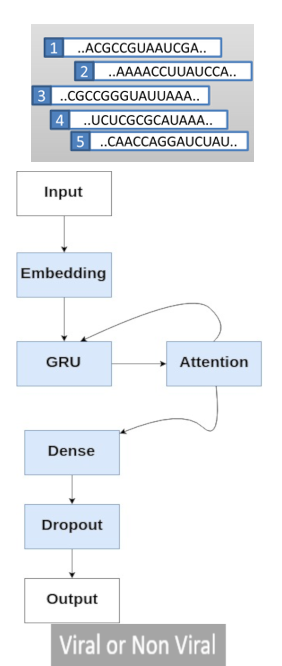
\includegraphics[width=\linewidth]{Pictures/model_diagram.PNG}
		\caption{Neural network model architecture} 
		\label{fig:model_diagram}
	\end{subfigure}
	\caption{VirNet model} 
	\label{fig:model_arch}
\end{figure}


% Chapter 4

\chapter{Experimental results} % Main chapter title

\label{Chapter4} % For referencing the chapter elsewhere, use \ref{Chapter1} 

\lhead{Chapter 4. \emph{Experimental results}} % This is for the header on each page - perhaps a shortened title

%----------------------------------------------------------------------------------------

\section{Data Generation}

\subsection{Building training and testing dataset}
We downloaded viruses, bacteria and archaea genomes from RefSeq database then we divided them randomly into a train and test genomes with 80\% of total base pairs in training. Table \ref{table:genome_stats} shows the number of genomes we used in training and testing. We processed all available viral genomes until Nov. 1, 2017 and a sample from prokaryotic genomes due to the huge number of available prokaryotic genomes. Then, we converted the viral genomes into non-overlapping fragments of different lengths n = \{100, 500, 1000, 3000\}. We generated an approximate number of non-overlapping fragments of prokaryotic genomes with the same lengths randomly as well. (Table \ref{table:fragments_stats}). We balanced the data of both classes using random under-sampling technique to avoid the bias to the majority class with the deep neural network. Figure \ref{fig:data_pipline} shows more details for data pipeline.

\begin{figure}[!htbp]
	\centering
	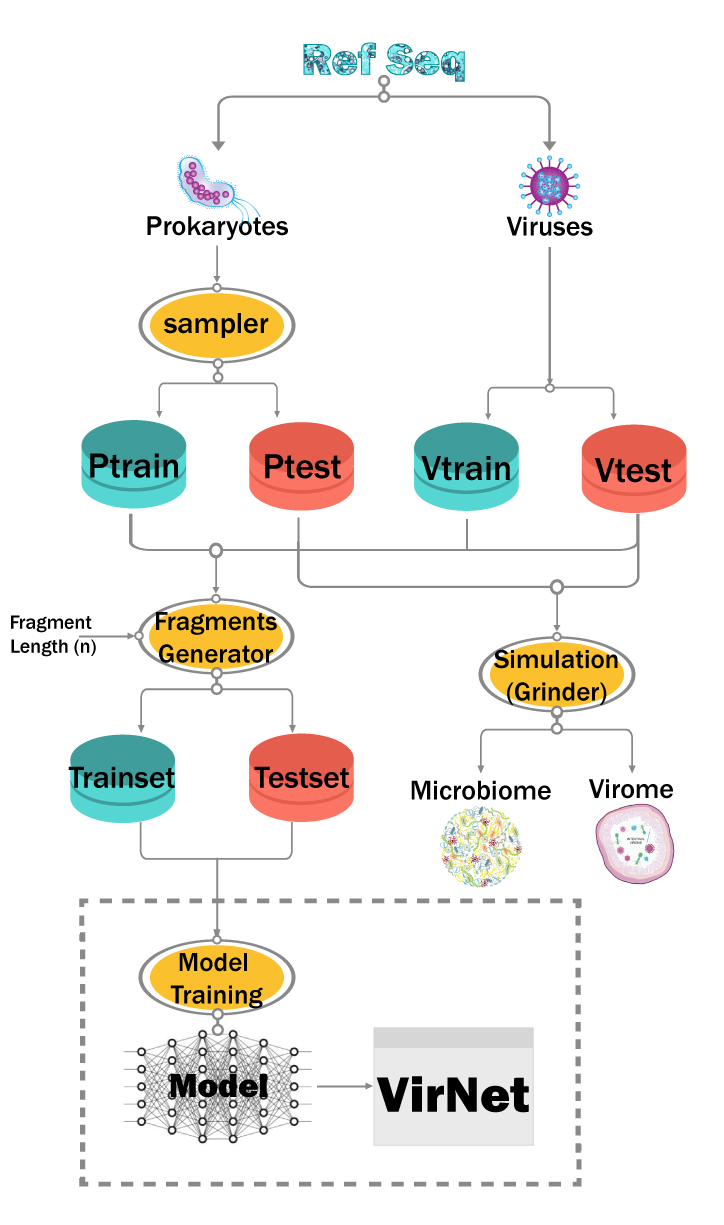
\includegraphics[width=\columnwidth]{Pictures/data_pipeline.PNG}
	\caption{VirNet Data Pipeline}
	\label{fig:data_pipline}
\end{figure}

\begin{table}[!htbp]
	\centering
	\begin{tabular}{||c c c c||} 
		Genome & Train & Test & Total \\ [0.5ex] 
		\hline\hline
		Viruses & 7686  & 1870 & 9556 \\ 
		Prokaryotes & 143241  & 35543 & 178784  \\ [1ex] 
	\end{tabular}
	\caption{The number of used genomes from RefSeq}
	\label{table:genome_stats}
\end{table}

\begin{table}[h!]
	\centering
	\begin{tabular}{||c c c||} 
		Fragment Length (N) & Train & Test \\ [0.5ex] 
		\hline\hline
		100 bp & 2088863  & 527020  \\ 
		500 bp & 420857  & 106168  \\
		1000 bp & 212253  & 53528  \\
		3000 bp & 73163  & 18425  \\ [1ex] 
	\end{tabular}
	\caption{The number of fragments generated from viruses genomes}
	\label{table:fragments_stats}
\end{table}

\subsection{Generating simulated virome and microbiome}
Grinder \cite{angly2012grinder} is an open-source tool commonly used for generating a simulate amplicon and shotgun metagenomic datasets from reference genomes. 
We generated two metagenomic data of virome and microbiome of 1M reads and fragment length 100bp using Grinder with our reference test genomes to simulate shotgun metagenomic sequences in order to verify the ability of our tool to detect viral reads in metagenomic data instead of generated fragments from the reference genomes. The virome data has 75\% of viral reads while microbiome has 25\%. Moreover, we used Illumina error model indicated by mutation\_dist poly4 3e-3 3.3e-8 and mutation ratio 91:9 (9 indels for each 91 substitution mutations) because for Illumina indel errors occur more often than substitution errors \cite{laehnemann2015denoising}. Table \ref{table:simulate_stats} shows simulated data statistics.  \\

\begin{table}[!htbp]
	\centering
	\begin{tabular}{||c c c||} 
		& Microbiome & Virome \\ [0.5ex] 
		\hline\hline
		Bacteria Length & 75450367  bp  & 17551396 bp  \\
		Bacteria Genomes & 1488 & 422\\
		Bacterial reads & 803742 & 176059\\
		Viruses Length & 25133078 bp  & 52609236 bp  \\ 
		Viruses Genomes & 845 & 1870\\
		Viral reads & 196258 & 823941 \\  
		Viral Ratio & 25.00\% & 75.00\% \\ 
		Library coverage &  0.994x &  1.001x  \\
		Diversity (richness) & 2302 & 2726 \\ [1ex]
	\end{tabular}
	\caption{Grinder Simulated Metagenome}
	\label{table:simulate_stats}
\end{table}


\subsection{Case Study: Real metagenomic data}
We applied our tool to two real metagenomes as a case study
\begin{enumerate}
	\item \textbf{454}: Subtropical freshwater microbial and viral metagenome (SRR648314).\
	\item \textbf{Illumina}: Lake Michigan virome (SRX995836).
\end{enumerate}
Our tool is able to read not only fasta files and fastq files. Furthermore, it is able to deal with paired-end reads i.e. if one of the two pairs is identified as a virus, the other should be the same. If there are conflicts between the classifications of the two pairs; this pair could be denoted as ambiguous.

\section{Results}
\subsection{Results for generated fragments}
We tested VirNet on different lengths of fragments n= \{100, 500, 1000, 3000\} from our testing set of viruses and prokaryotes RefSeq genomes. Moreover, we compared the output results to VirFinder results on the same training and testing data. VirNet predictions outperformed VirFinder for fragments with length 500, 1000 and 3000 (Figure \ref{fig:accuracy_graph}). The model reached to 82.82\% of accuracy whereas VirFinder tool obtained 75.61\%. Moreover, VirFinder can perdict the short fragments with length 100. Figures \ref{fig:roc_auc_virfindera} and \ref{fig:roc_auc_virneta} shows ROC-AUC curves of both tools on the testing set. Table \ref{table:virfinder_results} shows the comparison between both tools in terms of accuracy, average precision and average recall.

%\begin{table}[h!]
%	\centering
%	\begin{tabular}{||c l l l l l l l l||} 
%		Length(N) &	\multicolumn{2}{l}{Accuracy} & \multicolumn{2}{l}{Avg. Precision} & \multicolumn{2}{l}{Avg. Recall} &	\multicolumn{2}{l}{ROC-AUC} \\ [0.5ex] 
%		& VirNet & VirFinder & VirNet & VirFinder & VirNet & VirFinder & VirNet & VirFinder \\
%				\hline\hline
%		100 & 71.29\% &	63.9\%	& 0.72 & 0.64 & 0.71 & 0.64 & 0.80 & 0.64 \\
%		500 & 82.82\% &	75.61\% & 0.83 &	0.76 & 0.83 & 0.76 & 0.9 & 0.75 \\
%		1000 & 86.82\% &	80.28\% &  0.87 & 0.82 & 0.87 & 0.80 & 0.93 & 0.78 \\
%		3000 & 90.10\% &	87.11\% & 0.91 & 0.88 & 0.90 & 0.87 & 0.94 & 0.83\\[1ex]
%	\end{tabular}
%	\caption{VirFinder Results on our test-set}
%	\label{table:virfinder_results}
%\end{table}

\begin{table}[!htbp]
	\centering
	\begin{tabular}{||c l l l l l l||} 
		Length(N) &	\multicolumn{2}{l}{Accuracy} & \multicolumn{2}{l}{Avg. Precision} & \multicolumn{2}{l}{Avg. Recall}\\ [0.5ex] 
		& VirNet & VirFinder & VirNet & VirFinder & VirNet & VirFinder \\
		\hline\hline
		100 & 71.29\% &	63.9\%	& 0.72 & 0.64 & 0.71 & 0.64 \\
		500 & 82.82\% &	75.61\% & 0.83 &	0.76 & 0.83 & 0.76\\
		1000 & 86.82\% &	80.28\% &  0.87 & 0.82 & 0.87 & 0.80 \\
		3000 & 90.10\% &	87.11\% & 0.91 & 0.88 & 0.90 & 0.87 \\[1ex]
	\end{tabular}
	\caption{Comparison on fragments test-set}
	\label{table:virfinder_results}
\end{table}

\subsection{Results for simulated metagenomes}

As mentioned before, we tested VirNet on a simulated metagenomes of 100 bp and we found that VirNet performed much better than VirFinder. VirNet shows accuracy is 71.3\% on the virome data and 72.14\% on the microbiome data while VirFinder is 62.77\% on the virome data and 64.49\% on the microbiome data Table \ref{table:virfinder_results_simulated}). The ROC-AUC curves of both tools shows the difference between them (Figures \ref{fig:roc_auc_virfinderb} and \ref{fig:roc_auc_virnetb}).

\begin{figure}
	\centering
	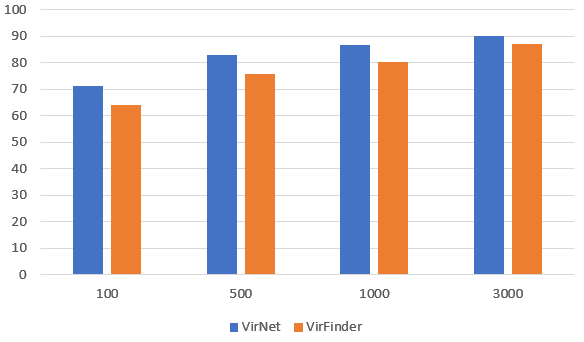
\includegraphics[width=\columnwidth]{Pictures/accuracy_graph.PNG}
	\caption{VirNet vs VirFinder Accuracy}
	\label{fig:accuracy_graph}
\end{figure}


\begin{figure}[!htbp]
	\centering
	\begin{subfigure}{0.5\textwidth}
		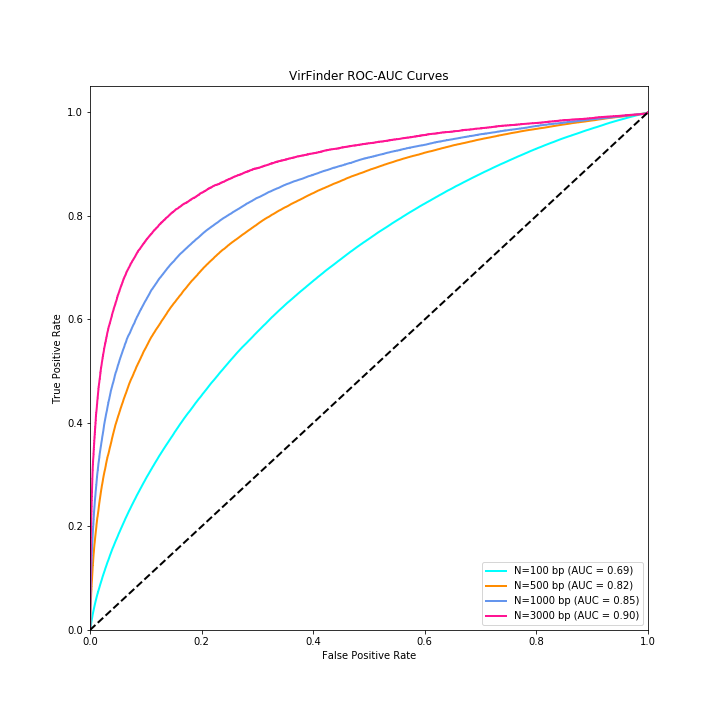
\includegraphics[width=\linewidth]{Pictures/roc_auc.png}
		\caption{VirFinder with generated fragments} 
		\label{fig:roc_auc_virfindera}
	\end{subfigure}
	\begin{subfigure}{0.5\textwidth}
		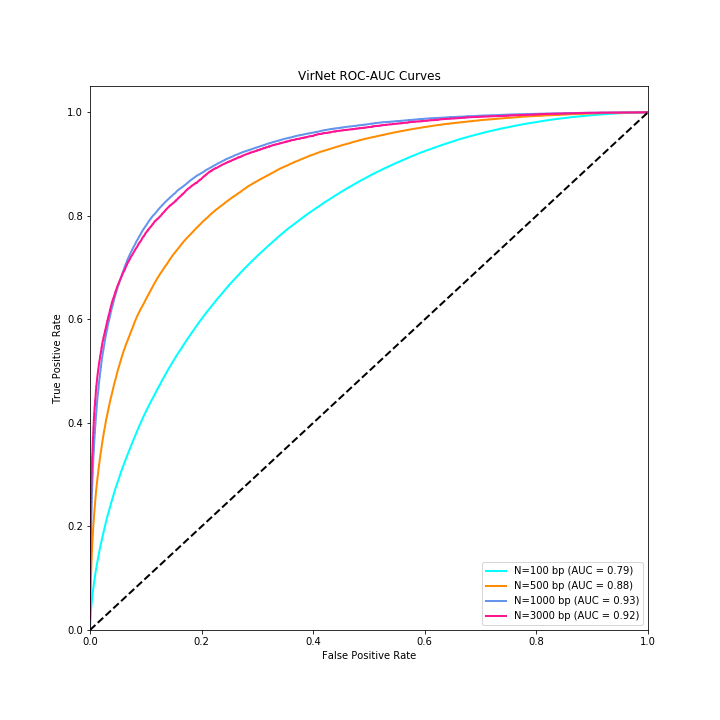
\includegraphics[width=\linewidth]{Pictures/virnet_roc_auc.png}
		\caption{VirNet with generated fragments} 
		\label{fig:roc_auc_virneta}
	\end{subfigure}
	\caption{ROC-AUC curves on fragments} 
	\label{fig:roc_auc_virfinder}
\end{figure}


\begin{figure}[!htbp]
	\centering	
	\begin{subfigure}{0.5\textwidth}
	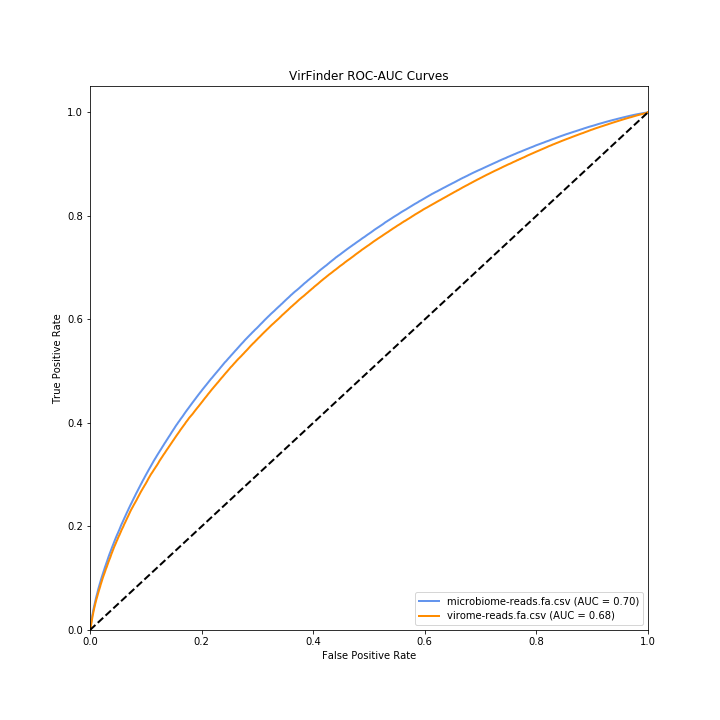
\includegraphics[width=\linewidth]{Pictures/roc_auc_simulated.png}
	\caption{VirFinder with simulated genomes} 
	\label{fig:roc_auc_virfinderb}
\end{subfigure}
\begin{subfigure}{0.5\textwidth}
	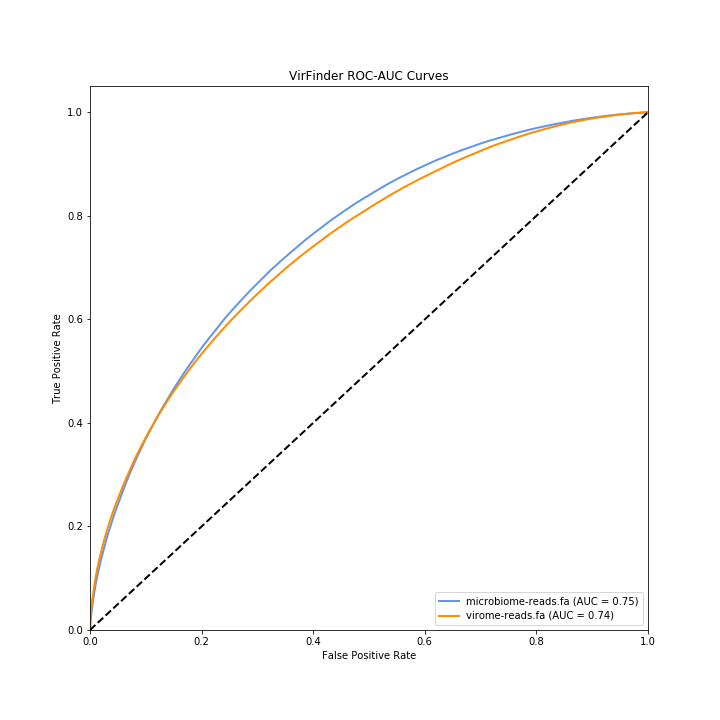
\includegraphics[width=\linewidth]{Pictures/virnet_roc_auc_simulated.png}
	\caption{VirNet with simulated genomes} 
	\label{fig:roc_auc_virnetb}

\end{subfigure}
		\caption{ROC-AUC curves on simulated metagenomes} 
		\label{fig:roc_auc_virfinder2}
\end{figure}

\begin{table}[!htbp]
	\centering
	\begin{tabular}{||l l l l l l l||} 
		Metagenome &	\multicolumn{2}{l}{Accuracy} & \multicolumn{2}{l}{Avg. Precision} & \multicolumn{2}{l}{Avg. Recall}\\ [0.5ex] 
		& VirNet & VirFinder & VirNet & VirFinder & VirNet & VirFinder \\
		\hline\hline
		Virome & 71.3\% &	62.77\%	& 0.71 & 0.63 & 0.72 & 0.62 \\
		Microbiome &	72.14\% & 64.49\% &	0.73 & 0.65 & 0.73 & 0.64 \\ [1ex]
	\end{tabular}
	\caption{Simulated Metagenomes Results}
	\label{table:virfinder_results_simulated}
\end{table}

\subsection{Results for real data}
we applied the tool on two real data with accession numbers SRR648314, SRX995836\_1 and SRX995836\_2. Table \ref{table:virnet_results_real} shows that our tool could able work on the real metagenomic data. 

\begin{table}[]
	\centering
	\begin{tabular}{||llll||}
		& SRR648314 & SRR1974517/1 & SRR1974517/2 \\
		\hline\hline
		Viral     & 39447     & 579697       & 590869       \\
		Non Viral & 20866     & 1055975      & 1044803      \\
		Total     & 60313     & 1635672      & 1635672     
	\end{tabular}
	\caption{VirNet results on real data}
	\label{table:virnet_results_real}
\end{table}

\subsection{VirNet processing speed}
Using GPUs is an advantage for our tool and make it very fast and scalable in processing massive amount of metagenomic reads simultaneously. The training process is around 5 hours with 2 million reads, while the prediction process is around 30 seconds on 1 million reads using Nvidia GeForce GTX 1080 Ti. On the other hand, VirFinder processing the reads on a single CPU less than VirNet by around 82 times. We can avoid that by using parallel CPU threads for VirFinder but in case you want to retrain it with new data, it will take a couple of days.

 
% Chapter 5

\chapter{Conclusion and Future Work} % Main chapter title

\label{Chapter5	} % For referencing the chapter elsewhere, use \ref{Chapter1} 

\lhead{Chapter 5. \emph{Conclusion and Future Work}} % This is for the header on each page - perhaps a shortened title

%----------------------------------------------------------------------------------------

\section{Summary}
Welcome to this \LaTeX{} Thesis Template, a beautiful and easy to use template for writing a thesis using the \LaTeX{} typesetting system.

If you are writing a thesis (or will be in the future) and its subject is technical or mathematical (though it doesn't have to be), then creating it in \LaTeX{} is highly recommended as a way to make sure you can just get down to the essential writing without having to worry over formatting or wasting time arguing with your word processor.

\LaTeX{} is easily able to professionally typeset documents that run to hundreds or thousands of pages long. With simple mark-up commands, it automatically sets out the table of contents, margins, page headers and footers and keeps the formatting consistent and beautiful. One of its main strengths is the way it can easily typeset mathematics, even \emph{heavy} mathematics. Even if those equations are the most horribly twisted and most difficult mathematical problems that can only be solved on a super-computer, you can at least count on \LaTeX{} to make them look stunning.

%----------------------------------------------------------------------------------------
\section{Conclusion}

\section{Future Work}

\begin{flushright}
Guide written by ---\\
Sunil Patel: \href{http://www.sunilpatel.co.uk}{www.sunilpatel.co.uk}
\end{flushright}
 
%\input{Chapters/Chapter6} 
%\input{Chapters/Chapter7} 

%----------------------------------------------------------------------------------------
%	THESIS CONTENT - APPENDICES
%----------------------------------------------------------------------------------------

\addtocontents{toc}{\vspace{2em}} % Add a gap in the Contents, for aesthetics

\appendix % Cue to tell LaTeX that the following 'chapters' are Appendices

% Include the appendices of the thesis as separate files from the Appendices folder
% Uncomment the lines as you write the Appendices

% Appendix A

\chapter{Appendix Title Here} % Main appendix title

\label{AppendixA} % For referencing this appendix elsewhere, use \ref{AppendixA}

\lhead{Appendix A. \emph{Appendix Title Here}} % This is for the header on each page - perhaps a shortened title

Write your Appendix content here.
%\input{Appendices/AppendixB}
%\input{Appendices/AppendixC}

\addtocontents{toc}{\vspace{2em}} % Add a gap in the Contents, for aesthetics

\backmatter

%----------------------------------------------------------------------------------------
%	BIBLIOGRAPHY
%----------------------------------------------------------------------------------------

\label{Bibliography}

\lhead{\emph{Bibliography}} % Change the page header to say "Bibliography"

\bibliographystyle{unsrtnat} % Use the "unsrtnat" BibTeX style for formatting the Bibliography

\bibliography{Bibliography} % The references (bibliography) information are stored in the file named "Bibliography.bib"

\end{document}  